\documentclass[11pt]{beamer}

\usepackage[utf8]{inputenc}
\usepackage[magyar]{babel}
\usepackage[T1]{fontenc}
\usepackage{lmodern}
\usepackage{zi4}
\usepackage{multirow}
\usepackage{listings}
\usepackage{ragged2e} % For \justifying command

\usetheme{Warsaw}

\renewcommand\UrlFont{\ttfamily\footnotesize}

% no navigation symbols
\setbeamertemplate{navigation symbols}{} 

% frame numbers
\expandafter\def\expandafter\insertshorttitle\expandafter{%
  \insertshorttitle\hfill%
  \insertframenumber\,/\,\inserttotalframenumber}

\author{Nagy András}
\title{Komponens-alapú UML modellek fordításának vizsgálata}
\date{2019. január}

\begin{document}

\begin{frame}
\titlepage
\end{frame}

\begin{frame}
	\frametitle{Komponens-alapú megközelítés}
	
	\begin{itemize}
		\item Program szereplőinek izolációja.
		\item A szereplők függetlenek a környezettől.
		\item Egymással interfész-portokkal kommunikálnak
	\end{itemize}
\end{frame}

\begin{frame}[fragile]
	\frametitle{Program szöveges modellezése}
	
	\begin{itemize}
		\item \textit{txtUML} keretrendszerben írjuk le a komponens-alapú modellt, Java-szerű nyelven, mely végrehajtható.
		\item Lefordítható egy szabványos UML2 modellre.
		\item A cél a kompozit struktúrák és akciók megfelelő UML2-es szabványának megtalálása, melyből hatékony C++ kód generálása.
	\end{itemize}
	
\end{frame}


\begin{frame}[fragile]
	\frametitle{Kompozit elemek bemutatása}	
	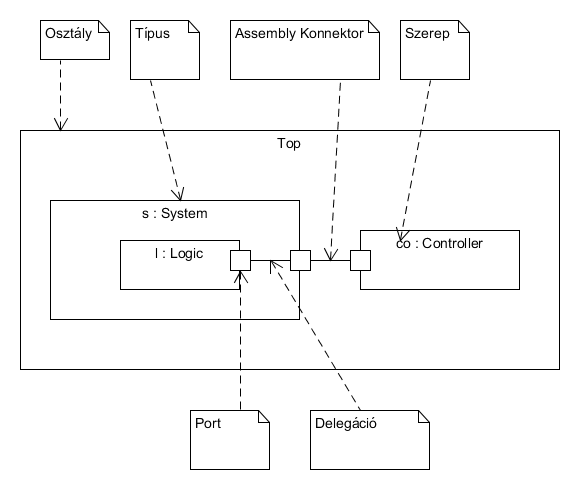
\includegraphics[scale=0.4]{composit_stuct_ea.png}
	
	Már az UML2-es reprezentáció sem triviális.

	
\end{frame}

\begin{frame}[fragile]	
	\frametitle{Főbb reprezentációs problémák}	
	\begin{itemize}
	\item Interfész port reprezentálása: mi a típusa, hogyan fejezzük ki az elvárt interfészt.
	\item Két port összekapcsolása futási időben.
	\item Porta való üzenetküldés.
	\end{itemize}
	
\end{frame}

\begin{frame}
	\frametitle{Interfész kódgenerálás stratégiái}
	
	\begin{itemize}
	\item Nincs interfész.
	\item A forráskód validációja kiszűrni a nem megengedett műveleteket.
	\item Triviális megoldás, nem kell kódgenerálási stratégia.
	\item Külső kommunikáció esetén olyan üzeneteket küldhetünk a porra, amit nem szabadna.
	
	\end{itemize}

\end{frame}

\begin{frame}
	\frametitle{Interfész kódgenerálás stratégiái}
	
	\begin{itemize}
	\item Jelző osztály generálása az interfész nevével.
	\item A fogadó műveletek szignáljai leszármaznak a jelző osztályból.
	\item A port \textit{send} művelete a jelző osztály leszármazottjait várja.	
	\end{itemize}

\end{frame}

\begin{frame}
	\frametitle{Interfész kódgenerálás stratégiái}
	
	\begin{itemize}
	\item Előbbi megoldás nem elég általános, portokra korlátozódik.
	\item Az interfész ne üres osztály legyen, hanem ő tartalmazza a \textit{send} műveleteket.
	\item Pontosan annyi különbözőt, ahány fogadó szignálja van.
	\item C++ sablon metaprogramozással leszűkíthetjük a kódot. (lásd diplomamunka) 	
	\end{itemize}

\end{frame}

\begin{frame}
	\frametitle{Interfész portok reprezentálása C++-ban}
	\begin{itemize}
	\item Bevezetünk egy port osztályt, sablonparaméterei az interfészek.
	\item Felveszünk minden porta egy port típusú adattagot a megfelelő interfészekkel.
	\item A portoknak két típusa lehet, a normál port, illetve az állapotgéppel összekapcsolt port.
	\item A normál port a befutó üzenetet egy gyerek felé továbbítja, az állapotgéppel összekapcsolt port a tartalmazó osztály állapotgépe felé.
	\item Ez más viselkedést és referencia tárolásokat jelent, melyeket leszármazással a legtisztább megoldani.
	\end{itemize}

\end{frame}

\begin{frame}
	\frametitle{Üzenetküldés UML-ben}
	\begin{itemize}
	\item Használjuk a \textit{SendObjectAction} \textit{OnPort} referenciáját.
	\item A szemantika a kontextustól függ: Ha az akció végrehajtója megegyezik a célobjektummal, akkor üzenet küldésről beszélünk. (belülről kifele továbbítjuk az üzenetet)
	\item Egyébként pedig üzenet fogadásról. (Kívülről befele továbbítjuk az üzenetet)
	\end{itemize}

\end{frame}

\begin{frame}
	\frametitle{Üzenetküldés C++}
	\begin{itemize}
	\item Interfész felosztása kintről illetve bentről jövő üzenetek megkülönböztetésére.
	\item A fent említett \textit{PSCS} szabvány szerinti szemantikának megfelelő művelet generálása. (\textit{send} vagy \textit{receive})
	\item Mi ennek a szemantikája, mit jelent ez C++-ban?
	\end{itemize}
\end{frame}

\begin{frame}[fragile]
	\frametitle{Portról jött üzenet feldolgozása C++-ban}
	\begin{itemize}
	\item Az üzenet az objektum üzenetsorához fut be.
	\item Azonban megjelöljük, hogy melyik portról érkezett.
	\item Állapot-átmeneteknél megadhatjuk, mely portokról érkezett üzenetek érdekesek számunka.
	\item Feldolgozáskor (esemény, állapot) alapján megkeressük a megfelelő átmenetet, és vizsgáljuk, hogy az átmenet lehetséges portjai között között ott van-e az üzenet portja.
	\end{itemize}

\end{frame}

\begin{frame}
	\frametitle{Konnektor, konnent UML-ben}
	\begin{itemize}
	\item A \textit{Connector} értelemszerű
	\item A problémás a \textit{connect} művelet
		\begin{itemize}
		\item Többféle megoldás, nincs \textit{connect} akció UML-ben
		\item A kapcsolatok az osztályszerkezet konstruálásakor jönnek létre.
		\item \textit{PSCS} szabvány szerint, ha nem adunk meg konstruktor művelet, az alapértelmezett konstrukciós stratégia \textit{DefaultConstructionStrategy} fog életbe lépni.
		\item A szerkezet nem mindig egyértelmű.
		\item A \textit{CreateLinkAction} segítségével összeköthetünk kért portot a konnektor típusa mentén (A típus asszociációt portok típusai alapján generálhatjuk).
		\end{itemize}
	\end{itemize}
\end{frame}

\begin{frame}
	\frametitle{Portok összekapcsolása C++-ban}
	\begin{itemize}
	\item A referencia tárolását választottuk.
	\item Probléma: assembly vagy delegációs kapcsolatban áll a referenciával?
	\item Megoldás: Csomagoljuk be a port referenciát egy kapcsolat osztályra, mely eldönti, hogy a kapcsolatban álló portnak mely műveletét kell meghívni üzenetküldés/üzenetfogadás esetén. Ennek leszármazással két típusa van, a \textit{DelegationConnect} illetve az \textit{AssemblyConnect} 
	\item \textit{connect} műveletnél ezeket a referenciákat kell kölcsönösen kitölteni, ahol megadhatjuk annak a konnektornak a típusát, mely szerint összekapcsolunk, ez validálja az összekapcsolás helyességét. 
	\end{itemize}
		
\end{frame}

\begin{frame}
	\frametitle{Összefoglalás, eredmények}
	\begin{itemize}
	\item Az UML kompozit szabvány alapos értelmezése, a megfelelő reprezentációk és szemantika megtalálása.
	\item C++ kódgenerálási stratégiák készítése.
	\item Szabványos modell generálása txtUML modell alapján, egy stratégia implementációja.
	\end{itemize}
\end{frame}

\begin{frame}
	\frametitle{Komponens-alapú UML modellek fordításának vizsgálata}
	\begin{center}
		\Large{Köszönöm a figyelmet!}
	\end{center}
\end{frame}

\end{document}
